% HEADER and settings -- do not change
\documentclass[final,a4paper]{aust_thesis}
\usepackage{definitions}
%%


% The set of languages we want to show
\lstloadlanguages{Python}

% one can select one...
\lstset{language=Python}
%%%%%%%%%%%%%%%%%%%%%%%%%%%%%%%%%%%%%%%%%%%%%%%
%%!!          THIS WILL BE CHANGED       !!%%%%

%%   FRONT MATTER
\submityear{%
2019%
}
\submitmonth{%
July%
}
\title{%
Sentiment Analysis Based on Social Media Data
}
\author{%
Kudzai Zishumba
}
\tutor{%
Prof. dr. Lehel Csat\'o\\
~\\
Faculty of Mathematics and Informatics,\hspace*{-3cm}\\
Babe\c{s} Bolyai University of Cluj-Napoca,\hspace*{-3cm}\\
Romania
}




\begin{document}


% begin approval page
\begin{figure}[h]
  \centering
  \pgfimage[width=0.7\linewidth]{images/logo_approval}
\end{figure}



\begin{center}
\large\textbf{Approval by}
\end{center}
\leavevmode\\
\leavevmode\\
\leavevmode\\
\leavevmode\\
\noindent
\textbf{Supervisor}\\
Surname:\\
First name:\\
Signature:\\
\\
\\
\\
\\
\noindent
\textbf{The head of department}\\
Surname:\\
First name:\\
Signature:\\


\vspace*{\fill}
\begingroup
\begin{center}
\tiny KM 10, Airport Road, Galadimawa. Abuja – Nigeria. P.M.B 681, Garki-Abuja. Tel: +234 (0) 9 291 6265 -7
www.aust.edu.ng
\end{center}
\endgroup
%%%% end approval page




\pagebreak
\vspace*{\fill}
\begingroup
\centering

COPYRIGHT \textcopyright 2019\\
KUDZAI ZISHUMBA\\
ALL RIGHTS RESERVED\\
 
\endgroup




%% ABSTRACT
\begin{abstract}%

Sentiment analysis has proven to be one of the most challenging tasks in natural language processing (NLP).
%
Many AI systems have been developed which can detect the polarity of a sentence (degree of positivity, neutrality or negativity). 
%
But more information such as the emotion of the author can be detected.
%
Our task here is to build an artificial agent – or an AI system – that is capable of detecting polarity in a document as well as the emotion of the author.
%
Generally speaking, sentiment analysis detects the polarity of the opinion based on the object/subject in discussion. But emotion detection can identify the particular “mood” of the author. Social platforms – such as Facebook, Twitter, IMDB, or comment sections from online newspapers – to name a few – can provide a huge corpus of – usually unlabeled or extremely sparsely labelled – content.
%
Using modern machine learning tools and the available computational power, an agent can analyze the content -- given usually as a list of messages – and detect the general emotion “within the message”. It must be capable of identifying subjects with unstable or “chaotic” mood that might require attention.

Our aim is to attempt detecting the underlying emotion as well as the polarity of a document. In this process we will make use of open source libraries and publicly available data sets. The program will be able to run locally, both in geographic and in cultural sense, and to analyze the results that were obtained.


~

This work is the result of my own activity. I have neither given nor received unauthorized assistance on this work.

\end{abstract}

% this command generates the titlepage
\maketitle

%%

% this command generates the table of contents
{ \baselineskip 1ex
  \parskip 1ex
  \tableofcontents
}

\listoffigures
% \addcontentsline{toc}{section}{\numberline{}List of Figures}
\cleardoublepage
%%%%%%%%%%%%%%%%%%%%%%%%%%%%%%%%%%%%%%%%%%%%%%%%%%%%%%%%%%%
%%%%%%%%%%    the structure of your thesis     %%%%%%%%%%%%


% the document is structured into LOGICAL parts:
%!TEX root = kudzai_thesis.tex
%%%%%%%%%%%%%%%%%%%%%%%%%%%%%%%%%%%%%%%%%%%%%%%%%%%%%%%%%%%%%%%%%%%%%%%
\chapter{Introduction}\label{ch:INTRO}
%%%%%%%%%%%%%%%%%%%%%%%%%%%%%%%%%%%%%%%%%%%%%%%%%%%%%%%%%%%%%%%%%%%%%%%

%%%%%%%%%%%%%%%%%%%%%%%%%%%%%%%%%%%%%%%%%%%%%%%%%%%%%%%%%%%%%%%%%%%%%%%
Sentiment analysis makes use of computational techniques to study peoples' emotions and opinions
on given topics. In recent years this field has attracted a lot of attention from both academia and industry, it comes with a lot of challenging research problems but has a wide range of applications.

Whenever we want to make a decision we must take into consideration the opinions of others, this is what makes opinions important. Both individuals and organizations who want to know the opinions of others benefit from this.

Prior to the web,  no computational study on peoples opinions was being done. Opinionated text did not exist in abundance. To get peoples opinion one would typically need to use techniques such as surveys or questionnaires to get opinions from the public or simply ask from friends and or family members.
When organizations wanted to get opinions about services or products they would typically use these methods.   

But due to the explosive growth of social media websites and mobile applications, opinionated content on the web has increased exponentially. People can now share their opinions about almost anything on blogs, comment sections and social websites\cite{ref47}







%!TEX root = kudzai_thesis.tex
%%%%%%%%%%%%%%%%%%%%%%%%%%%%%%%%%%%%%%%%%%%%%%%%%%%%%%%%%%%%%%%%%%%%%%%
\chapter{Basics of Sentiment analysis}\label{ch:THEORY}

There are two approaches to sentiment analysis: lexicon-based and machine learning-based.
%
Machine learning as the name suggests requires the model to be trained, lexicon based consists of a set of rules and doesn’t require prior training, a third method although not used very often is a hybrid method that combines both lexicon and machine learning approaches, generally it yields better results than either method individually.\cite{ref2}
%
Table~\ref{tab:sent_analysis_approaches} will summarize the differences between the two approaches.

\begin{table}[h]
  \centering
  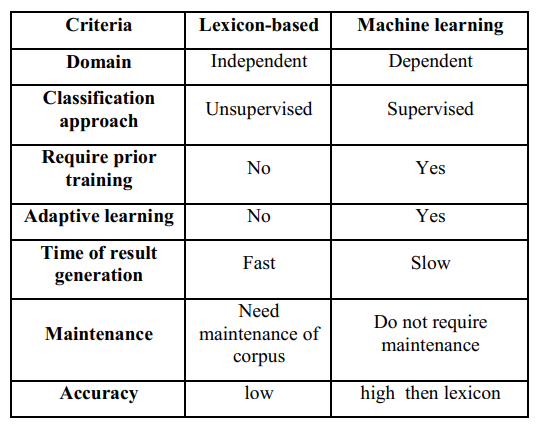
\includegraphics[width=0.5\linewidth]{images/lex_vs_ml.png}
  \caption{Comparison between lexicon and machine learning}
  \label{tab:sent_analysis_approaches}
\end{table}

Currently Sentiment analysis techniques seek to classify text as either positive, negative or neutral, using methods in Natural language processing (NLP). The common approach implemented involves statistical analysis and machine learning methods.\cite{ref2}

%
However people often express a particular emotion towards a certain topic. Specific emotions such as anger can lead to social unrest. This is undesirable but it can be helpful if we are able to quickly detect this before it occurs.
%
The proposed system will be a hybrid system it will use both machine learning approach as well as lexicon-based approach to detect both sentiment polarity and emotion.


\clearpage



\section{Lexicon (VaderSentiment)}
A lexicon is a collection of information about the words of a language about the lexical categories to which they belong. Lexicon based sentiment analysis makes use of labeled text this is very useful in detecting sentiment by emoticons. 
%
VaderSentiment is a python library that can be used to achieve this.\\ \\
VADER (Valence Aware Dictionary and sEntiment Reasoner) is a lexicon and rule-based sentiment analysis tool that is specifically attuned to sentiments expressed in social media.
VADER makes use of sentiment lexicon, which is a list of lexical features such as words, these words are labeled according to their sentiment polarity, positive, neutral or negative.
 \\ \\
An emoticon, short for "emotion icon", also known simply as an emote, is a pictorial representation of a facial expression using characters usually punctuation marks, numbers and letters to express a person's feelings or mood, or as a time-saving method rather than to type out a whole word, an emoticon can be used to convey the writer's feelings or intended tone. \\ \\

Some key features of Vader sentiment are: -

\begin{enumerate}

\item
Punctuation: The use of an exclamation mark(!), increases the magnitude of the intensity without modifying the semantic orientation. For example, “The food here is good!” is more intense than “The food here is good.” and an increase in the number of (!), increases the magnitude accordingly.

\item
Capitalization: Using upper case letters to emphasize a sentiment-relevant word in the presence of other non-capitalized words, increases the magnitude of the sentiment intensity. For example, “The food here is GREAT!” conveys more intensity than “The food here is great!”
\item
Degree modifiers: Also called intensifiers, they impact the sentiment intensity by either increasing or decreasing the intensity. For example, “The service here is extremely good” is more intense than “The service here is good”, whereas “The service here is marginally good” reduces the intensity.
\item
Conjunctions: Use of conjunctions like “but” signals a shift in sentiment polarity, with the sentiment of the text following the conjunction being dominant. “The food here is great, but the service is horrible” has mixed sentiment, with the latter half dictating the overall rating.
\item
Preceding Tri-gram: By examining the tri-gram preceding a sentiment-laden lexical feature, we catch nearly 90\% of cases where negation flips the polarity of the text. A negated sentence would be “The food here isn’t really all that great”.
\end{enumerate}

\clearpage
\subsection{Subjectivity and Objectivity (TextBlob)}
Subjectivity and objectivity differentiates opinionated and factual based text.\cite{ref2}
Being able to detect subjectivity and objectivity is an important part of sentiment analysis, because it can tell us more about the authors emotions and intentions, a subjective person is more likely to invoke action than an objective person. TextBlob python library can be used to detect the degree of subjectivity and the degree of objectivity, these results together with the polarity scores will be used to determine the impact of the sentiment. 

\clearpage
\subsection{Multi-label convolutional neural network text classifier (Spacy)}

SpaCy is a free, open-source library for advanced Natural Language Processing (NLP) in Python \\
Spacy makes use of a neural network text classifier. SpaCy can be used to categorize documents into the different emotion classes.
The Neural network is trained using stochastic gradient descent where the estimate of the error used to update the weights is calculated based on a subset of the training dataset. \\


\begin{figure}[h]
  \centering
  \pgfimage[width=0.7\linewidth]{images/sgd}
  \caption[Stochastic Gradient decent]%
  {Stochastic Gradient decent}
  \label{fig:ALAP:sm3}
\end{figure}






A SpaCy model uses statistical decisions to make predictions, the decision is based on examples used to train the model. Training the model requires training data, training data is: examples of text with the labels that we want to predict. This will be in the following categories
\begin{itemize}
\item "anger"
\item "disgust"
\item "fear"
\item "sadness"
\item "shame"
\item "joy"
\item "guilt"
\end{itemize}




The following diagram shows how SpaCy model is trained

\begin{figure}[h]
  \centering
  \pgfimage[width=0.7\linewidth]{images/spacy_training}
  \caption[SpaCy Training]%
  {SpaCy Training:https://spacy.io/usage/training}
  \label{fig:ALAP:sm3}
\end{figure}
 
\clearpage

\subsection{Training Dataset (ISEAR)}


Robert Plutchik invented a wheel of emotions. He suggested eight primary emotions: joy opposite to sadness. Similarly, anger opposite to fear; trust opposite to disgust and surprise opposite to anticipation. These four opposite emotion pairs, show the 8 basic emotions. Additionally, Plutchik’s model shows connections between the ideas of circle of emotions using a color wheel. Like the case of colors, primary emotions can also be expressed at different degrees of their intensities, for each emotion there are three degrees. For example, serenity is a less intense degree of joy
and ecstasy is a more intense degree of joy. Plutchik’s emotions can be mixed with one another
forming a new different emotion. For example, combination of joy and trust resulted to form a new
emotion ‘love’. Likewise, joy, anger and trust are combined and form jealousy\cite{ref:4}.

\begin{figure}[h]
  \centering
  \pgfimage[width=0.7\linewidth]{images/emotion_wheel}
  \caption[Robert Plutchik's wheel of emotions]%
  {Robert Plutchik's wheel of emotions}
  \label{fig:ALAP:sm3}
\end{figure}


ISEAR (International Survey on Emotion Antecedents and Reactions) is an open dataset collected by Klaus R. Scherer and Harald Wallbott. 
ISEAR dataset contains seven major emotions based on Robert Plutchik's wheel of emotions : joy, fear, anger, sadness, disgust, shame, and guilt.\\
It has over 7,600 entries for the emotion classes. This will be a good training dataset for emotion detection.
\clearpage

\subsection{Streaming twitter (tweepy)}
Tweepy is an open source python library that can be used to stream tweets from twitter in real time through the Twitter API.


\subsection{Confusion matrix}
A confusion matrix is used in machine learning to determine the performance of a classification algorithm. It is a tabular form than compares test data for which its true values are known. I will use the confusion matrix to evaluate the performance of my classification model.

A confusion matrix consists of the following classes.
 \begin{itemize}

\item
true positives (TP): This is when we have given a correct positive prediction

\item
true negatives (TN): This is when we have given a correct negative prediction.

\item
false positives (FP): This is when we have predicted yes, but the true value is no

\item
false negatives (FN): This is when we have predicted no, but the true value is yes

\end{itemize}

\begin{figure}[h]
    \centering
    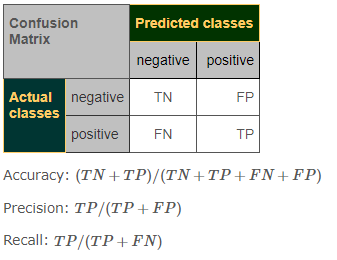
\includegraphics{images/confusion_matrix.png}
    \caption{Confusion matrix}
\end{figure}

  The above table shows how to determine the accuracy of the prediction using a confusion matrix. However, there are problems with accuracy. It assumes equal costs for both kinds of errors that is to say it assumes that we have an equal number of positives and negatives. A 99\% accuracy can either be excellent, good, mediocre, poor or terrible depending upon the problem
\clearpage
In the case of having multiple classes the confusion matrix becomes


\begin{figure}[h]
    \centering
    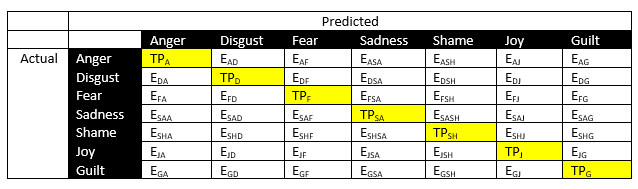
\includegraphics{images/confusion_matrix_2.png}
    \caption{Confusion matrix with multiple classes}
\end{figure}

Things to notice about a confusion matrix with multiple classes
\begin{itemize}
\item \textbf{total number of test examples} of any class if given by the sum of the corresponding row \textbf{(i.e TP + FN)}
\item \textbf{Total number of False Negatives} for a class is the sum of values in the corresponding row excluding the \textbf{True positives}

\item \textbf{Total number of false positives} for a class is the sum of values in the corresponding column excluding the \textbf{true positives}

\item \textbf{Total number of true negatives} for a certain class will be the sum of all columns and rows  excluding that classes column and row
\end{itemize}
  
\textbf{Accuracy} calculated as the sum of correct classifications divided by the total number of classifications\\
\textbf{Precision} is calculated as \textbf{ TP/(TP+ FP)}\\
\textbf{Recall} also called sensitivity, corresponds to the tue positive rate of the considered class
\\
calculated as Recall=Sensitivity=TP/(TP+FN)

\clearpage



\chapter{Sentiment analysis}

\subsection{Implementing (VaderSentiment and TextBlob)}


Using \textbf{"VaderSentiment"} library. Using an analyzer object, and looping through the list of tweets  calling the analyser.polarity\_scores() method and appending the results to an array.

\begin{lstlisting}
from vaderSentiment.vaderSentiment import SentimentIntensityAnalyzer
analyser = SentimentIntensityAnalyzer()#create the vader sentiment analyser object
sentiment_vs_tweets=[]#array will hold the processd tweets with the sentiment and objective labels
index=0
for t in tweets:
    sentiment_vs_tweets.append( analyser.polarity_scores(t) )#add the processed tweet to the list
    print(sentiment_vs_tweets[index])#print the sentiment polarity and subjecivity
    index=index+1
\end{lstlisting}


The above code will produces the following results

\begin{lstlisting}
{'neg': 0.252, 'neu': 0.581, 'pos': 0.168, 'compound': -0.3182}
{'neg': 0.0, 'neu': 1.0, 'pos': 0.0, 'compound': 0.0}
{'neg': 0.194, 'neu': 0.806, 'pos': 0.0, 'compound': -0.5574}
{'neg': 0.0, 'neu': 1.0, 'pos': 0.0, 'compound': 0.0}
{'neg': 0.194, 'neu': 0.806, 'pos': 0.0, 'compound': -0.5574}
\end{lstlisting}




Using \textbf{TextBlob} to detect the degree of subjectivity and objectivity of the documents.


\begin{lstlisting}
#here we use TextBlob python library to detect sentence/tweet/document polarity as well as subjectivity and store the results
#textblob uses a machine learning approach
from textblob import TextBlob
sentiment_tb_tweets=[]#array will hold the processd tweets with the sentiment and objective labels
index=0
for t in tweets:
    sentiment_tb_tweets.append( TextBlob(t) )#add the processed tweet to the list
    print(sentiment_tb_tweets[index].sentiment)#print the sentiment polarity and subjecivity
    index=index+1
    
sentiment_tb_tweets[0].subjectivity
\end{lstlisting}


The above code produces the following results


\begin{lstlisting}[language=Python]
Sentiment(polarity=0.0, subjectivity=0.25)
Sentiment(polarity=0.14285714285714285, subjectivity=0.31785714285714284)
Sentiment(polarity=0.0, subjectivity=0.06666666666666667)
Sentiment(polarity=0.2, subjectivity=0.2)
Sentiment(polarity=0.0, subjectivity=0.06666666666666667)
\end{lstlisting}

\clearpage

\subsection{Training SpaCy Text classifier}
Using the ISEAR training data
We can train a SpaCy model to classify text into some categories
\begin{figure}[h]
  \centering
  \pgfimage[width=0.5\linewidth]{images/isear}
  \caption{Sample ISEAR training dataset with labels}
  \label{fig:ALAP:sm1}
\end{figure}

We begin training the SpaCy model on the above training set,
start by reading in the data 
\begin{lstlisting}
nlp    = spacy.load('en_core_web_sm')#load english model
file    = open("data/train_data.txt","r")#read in training set from text file uses pipe delimiter
#read in the training set with the labels
for row in f_data:
    train_data.append( (row.split('|')[0],\
                        {"cats":\
                         {\
                          "anger"    :int(row.split('|')[1]),\
                          "disgust"  :int(row.split('|')[2]),\
                          "fear"     :int(row.split('|')[3]),\
                          "sadness"  :int(row.split('|')[4]),\
                          "shame"    :int(row.split('|')[5]),\
                          "joy"      :int(row.split('|')[6]),\
                          "guilt"    :int(row.split('|')[7])\
                        }}) )
                        
\end{lstlisting}
\clearpage
We then update the nlp model with the new training set
\begin{lstlisting}
#create the spacy nlp pipeline
textcat = nlp.create_pipe('textcat')
#add the pipeline to the nlp model| last=true since we want to add these conponents at the end of the model
nlp.add_pipe(textcat, last=True)
#declare the lables/categories
textcat.add_label('anger')
textcat.add_label('disgust')
textcat.add_label('fear')
textcat.add_label('sadness')
textcat.add_label('shame')
textcat.add_label('joy')
textcat.add_label('guilt')

optimizer = nlp.begin_training()
#next we will update the model with our own train_data from the csv file
for itn in range(1):
    for doc, gold in train_data:
        random.shuffle(train_data)
        losses = {}
        index = 0
        for text, annotations in train_data:
            nlp.update([doc], [gold], sgd=optimizer, drop=0.45, losses=losses)#drop rate at .45
            print("Iteration: {0}, %{1:.2f} Complete".format((itn+1), index/len(train_data) * 100))#show the progress
            index += 1
        print(losses)
 
\end{lstlisting}


After training the model we can now run some tweets via the model 
\begin{lstlisting}
#determine the class of the tweets using the spacy model trained earlier
#create a document and run it thru the nlp pipeline 
classified_tweets = []#array will hold the spacy classified tweets
index=0
for t in tweets:
    classified_tweets.append(  nlp(t) )
    print( classified_tweets[index].cats )#print the categories/classes of the document
    index=index+1  
\end{lstlisting}

The above code produces the following results
\begin{lstlisting}
{'anger': 0.8638094067573547, 'disgust': 0.41107258200645447, 'fear': 0.007243141997605562, 'sadness': 0.04211084172129631, 'shame': 0.7023115158081055, 'joy': 0.6675902605056763, 'guilt': 0.9010916352272034}
{'anger': 0.7449342012405396, 'disgust': 0.4830150306224823, 'fear': 0.016353892162442207, 'sadness': 0.2870638370513916, 'shame': 0.40636202692985535, 'joy': 0.1324012577533722, 'guilt': 0.41464924812316895}
{'anger': 0.7480689883232117, 'disgust': 0.4755619764328003, 'fear': 0.035106029361486435, 'sadness': 0.1592441201210022, 'shame': 0.4828783869743347, 'joy': 0.16910341382026672, 'guilt': 0.4793942868709564}
{'anger': 0.7859129905700684, 'disgust': 0.47182315587997437, 'fear': 0.026509756222367287, 'sadness': 0.32458046078681946, 'shame': 0.12689484655857086, 'joy': 0.23759214580059052, 'guilt': 0.9908844828605652}
{'anger': 0.7480689883232117, 'disgust': 0.4755619764328003, 'fear': 0.035106029361486435, 'sadness': 0.1592441201210022, 'shame': 0.4828783869743347, 'joy': 0.16910341382026672, 'guilt': 0.4793942868709564}
\end{lstlisting}

SpaCy model is able to classify the class of the text based on our training set



\clearpage

\subsection{Streaming twitter API(Tweepy)}

The python library tweepy can support accessing Twitter via Basic Authentication and the newer method, OAuth. The API parameters allow filtering tweets based on language, geolocation and tweets containing a particular word or phrase.

\begin{lstlisting}
auth   = OAuthHandler(consumer_key, consumer_secret)
auth.set_access_token(access_token, access_token_secret)

stream = Stream(auth, listner)
#run this code async 
streamer=stream.filter(track=search_terms,is_async=True,languages=langs,locations=loca_tions)
\end{lstlisting}

The listener object is a class that inherits from StreamListener class, it listens for any incoming tweets, cleans the tweets and then stores them in an array.

\begin{lstlisting}
class StdOutListener(StreamListener):
    def on_data(self, data):
        obj = json.loads(str(data))#convert the tweet into a json format
        #clean the tweets before inserting into the array
        clean_tweet = remove_pattern(obj["text"],"@[\w]*")#remove twitter handles (@user)
        clean_tweet = clean_tweet.replace("[^a-zA-Z#]", " ")#replace puntuation marks
        clean_tweet = clean_tweet.replace("RT :","")#replace the re tweet symbol
        clean_tweet = re.sub('http[s]?://(?:[a-zA-Z]|[0-9]|[$-_@.&+]|[!*\(\),]|(?:%[0-9a-fA-F][0-9a-fA-F]))+', '', clean_tweet, flags=re.MULTILINE)#remove hyperlinks
        
        score       = vs_analyser.polarity_scores(clean_tweet)
        sentiment_polarity_scores.append( float(score["compound"]) )#append the sentiment score to the array
        sentiment_tb_tweets.append( TextBlob(clean_tweet) )#append the texblob object to the array
        sentiment_vs_tweets.append( nlp(clean_tweet) )#append the vader sentiment object to the array
        tweets.append(clean_tweet)#append the clean tweet to the list of tweets
\end{lstlisting}



%%%%%%%%%%%%%%%%%%%%%%%%%%%%%%%%%%%%%%%%%%%%%%%%%%%%%%%%%%%%%%%%%%%%%%%
\subsection{Evaluating SpaCy classification model}\label{sec:THEORY:linear}
Because of the huge size of the training dataset, using the whole data set to train and evaluate the model would take too long. The solution therefore is to use a small sample of the dataset to train and evaluate.
The training set has 23 samples and the evaluation set has 8 samples.\\
The following is the results of the evaluation based on the confusion matrix.

\begin{lstlisting}
Accuracy:  1.4285714285714286



Precision_anger:  0.6666666666666666
Precision_disgust:  1.0
Precision_fear:  0.4
Precision_sadness:  1.0
Precision_shame:  1.0
Precision_joy:  1.0
Precision_guilt:  1.0
Total_Precision:  0.8666666666666666



Recall_anger:  1.0
Recall_disgust:  0.6666666666666666
Recall_fear:  1.0
Recall_sadness:  0.5
Recall_shame:  0.5
Recall_joy:  0.5
Recall_guilt:  0.5
Total_Recall:  0.6666666666666666
\end{lstlisting}

The results for each individual classification is quite satisfactory, considering that the training set and evaluation set is considerably small. Both the precision and the Recall is 50\% and above.






\appendix
%!TEX root = kudzai_thesis.tex



{ 
  \renewcommand{\baselinestretch}{0.8}\normalsize %
  \setlength{\itemsep}{-2.4mm}
  \setlength{\bibspacing}{0.67\baselineskip}
  \bibliographystyle{abbrvnat}
  \setcitestyle{numbers}
  \bibliography{thesis}
}

\end{document}
